\chapter{Background Theory}
\label{chp:theory} 

\section{Introduction}

This chapter will provide the background theory which is necessary to understand the implementation described in chapter \ref{chp:implementation}. Section \ref{sec:terminology} introduces some robot terminology and concepts. Section \ref{sec:ros} provides a thorough introduction to \ac{ROS}, which is the framework of choice in this implementation. Next, follows a section on sensors. More specifically the Kinect for Xbox 360 and a \ac{LIDAR}, URG-04LX-UG01. The two final sections provide basic insight into \ac{SLAM} and autonomous navigation in \ac{ROS} respectively. 

%\section{Modelling and Simulation}
%\label{sec:modelling}
\subsection{Brief Introduction to Robot Terminology}
\label{sec:terminology}

\subsubsection{Joints and Links}

A robot can be described by a set of rigid \textit{links} connected to each other by \textit{joints}. A link is described by a set of kinematic attributes based on its shape and mass. A joint between two links describe the freedom of movement between the coordinate systems of each link. When a set of links and joints are put together, they will define the kinematic tree of the robot, i.e. how the robot and its components can move. Typical joint classes are:

%\begin{description}[align=right]
%	\item[Static] Transforms between links are constant.
%	\item[Revolute]  A rotary motion between the links. Like a door hinge or a knee.
%	\item[Prismatic] A linear motion between the links. 
%	\item[Continous] Unbounded rotary motion. Typically used for rotating wheels.	
%\end{description}

\begin{center}
	\begin{tabular}{ r p{10cm} }
	\textbf{Static} & Transforms between links are constant.\\
	\textbf{Revolute} &  A rotary motion between the links - like a door hinge or a knee.\\
	\textbf{Prismatic} & A linear motion between the links. \\
	\textbf{Continous} & Unbounded rotary motion. Typically used for rotating wheels. \\
	\end{tabular}
\end{center}

\subsubsection{Coordinate Systems and Poses}

\subsubsection{Mobile Bases}



\subsection{Simulating in Gazebo}

\section{ROS}
\label{sec:ros}
\subsection{Introduction}

The \ac{ROS} is a collection of software libraries, tools and drivers intended for robot software development. A \ac{ROS} installation can be tailored to meet the demands of a wide range of robots with varying complexity. \ac{ROS} is usually installed in the form of an already built Debian-package. These packages are only compatible with a few versions of Ubuntu which are specified on the \ac{ROS} homepage. When installed and configured, \ac{ROS} will run on top of Linux, and can be perceived as and extention of Linux itself. Installing \ac{ROS} from source is possible, but not recommended \cite{ROS_install}.

Historic roots of \ac{ROS} can be traced back to Stanford University at the beginning of the 2000s. At Stanford, several robotics software frameworks, including \ac{STAIR} and the \ac{PR} program, were created to provide dynamic, flexible and well tested foundations for further robot development and research. In 2007, a nearby start-up company and robot incubator, Willow Garage, sought to build upon these concepts, and initiated a collaborative and open development process of a new software framework. This framework eventually became \ac{ROS}\cite{ROS_history}\cite{rosbook15}. The framework can be used under the BSD open-source license\cite{BCD_license}. Today, \ac{ROS} comes in many forms and comprise hundreds of advanced packages, algorithms and drivers, making it applicable for hobbyists, industrial automation, research and everything in between. 

\subsection{Important ROS Concepts}
\label{sec:ros_concepts}
The following descriptions are included in order to provide a complete, self-contained description of the project implementation. Similar descriptions can be found on the official \ac{ROS} website\footnote{\url{http://www.ros.org/}}, as well as in any book on \ac{ROS} (for example \cite{rosbook15} or the more comprehensive \cite{koubaa2016robot}). 

\subsubsection{The ROS Graph}

A \ac{ROS} system comprise a set of small programs that communicate with each other through messages. These programs become nodes in the \ac{ROS} graph. The nodes communicate with each other by publishing and subscribing to topics that form the edges of the graph. A topic must have the format of one of the specific data types provided by \ac{ROS}. For example, a node which receives temperature data from a thermometer, may publish the data as a topic on the \ac{ROS} system with the type \texttt{sensor\_msgs/Temperature}. There are many other data formats, e.g. velocity messages, \texttt{geometry\_msgs/Twist}; images, \texttt{sensor\_msgs/Image}; odometry messages, \texttt{nav\_msgs/Odometry} and so on. Each node in the graph are typically POSIX processes, and the edges are TCP connections\cite{rosbook15}. A minimal example of a graph is shown in figure \ref{fig:minimum_graph}.

\begin{figure}[h]
    \centering
    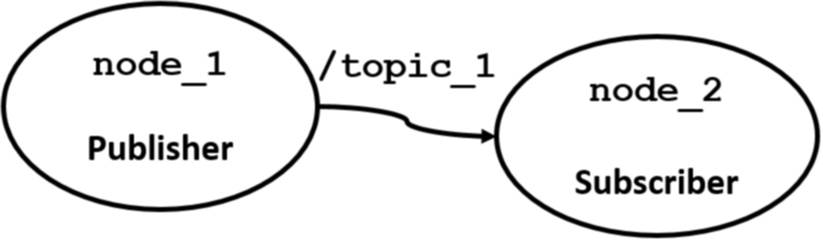
\includegraphics[width=0.8\textwidth]{minimum_graph_bl}
    \caption{A minimal \ac{ROS} graph. There are two nodes, \texttt{node\_1} and \texttt{node\_2}. \texttt{node\_1} publishes data, i.e. a topic, by the name \texttt{topic\_1}. \texttt{node\_2} can receive the data by subscribing to \texttt{topic\_1}.}
    \label{fig:minimum_graph}
\end{figure}

\subsubsection{roscore}

\texttt{roscore} is an essensial part of any \ac{ROS} system as it enables nodes to communicate with each other. An instance of \texttt{roscore} must be started before launching any nodes. When a node is started, it will inform \texttt{roscore} of which topics it publishes and which topics it wish to subscribe to. Then, \texttt{roscore} will provide the information which allows the node to form a peer-to-peer connection to other nodes.

\subsubsection{tf}

\texttt{tf}\cite{tf_paper} is a coordinate system transformation library used in \ac{ROS}. Parts of a \ac{ROS} system can listen to broadcasted transforms in the form of messages, \texttt{tf/tfMessage}, which describe a coordinate system transform between one or more parent-child link pairs. \texttt{tf} also provides timing information it the messages. This is a very important feature because a node may depend on synchronized sensor streams with many different coordinate frames. Comparing a laser scan with a point clout that was received seconds ago may lead to errors. 

\subsubsection{Project Structure and the \textit{catkin} Build System}
\label{sec:catkin}
The source code in a \ac{ROS} system is organized into packages. Each package provides a specific functionality to the system. Some packages can be downloaded and installed from a remote repository, while other packages will be created by the in-house developers for their specific robotic system. In this project, locally created ROS-packages were placed into a \textit{catkin workspace}. This workspace contains the  original source code and build specifications. Details are provided in chapter \ref{chp:implementation}. As presented in\cite{ROS_tut_pkg}, a general workspace structure is as follows:

\begin{verbatim}
workspace_folder/        -- CATKIN WORKSPACE
  src/                   -- SOURCE SPACE
    CMakeLists.txt       -- 'Toplevel' CMake file, provided by catkin
    package_1/
      CMakeLists.txt     -- CMakeLists.txt file for package_1
      package.xml        -- Package manifest for package_1
    ...
    package_n/
      CMakeLists.txt     -- CMakeLists.txt file for package_n
      package.xml        -- Package manifest for package_n
\end{verbatim}

A \ac{ROS} project will usually utilize the catkin build system.

\subsubsection{\texttt{roslaunch}}

\texttt{roslaunch}\cite{ROS_launch} is a \ac{ROS} package tool used to launch multiple nodes from a single command line. This is useful for larger projects with many nodes, interactions and parameters. Exactly which nodes to launch is defined in XML-files with the \textit{.launch} extension. In a launch file, the developer can group nodes together, pass arguments to the nodes and launch other launch files. Launch files can be launched from the command line as follows:

\begin{verbatim}
$ roslaunch <package name> <launch file name>.launch <argument1>:=true
\end{verbatim}

\subsection{An Overview of ROS-Related Tools}

\subsubsection{Robot Modelling In URDF}

\ac{URDF} is an XML-like format for describing robots. The robot description is made up of links and joints. Each link description contains information of, e.g., its shape, inertial tensor, collision boundaries. The links are connected to each other by joints.

\subsubsection{Visialization in \texttt{rviz}}

\texttt{rviz} is an invaluable tool for visualizing on-line robot behavior. Simply put, \texttt{rviz} is created to visualize what the robot sees, and how it plans ahead. Many of the images in the following chapters were obtained in \texttt{rviz}. 

\subsubsection{Simulation in Gazebo}


\subsection{Notable Robots Running ROS}

\paragraph{PR2 - Personal Robot 2}

PR2, developed by Willow Garage is one of the first robots designed to run \ac{ROS} \cite{rosbook15}, and also one of the most advanced and capable robots with \ac{ROS} today. PR2 is build for research and development of service robot applications. The navigation stack used in this thesis has been tested on the PR2. \cite{tbd} describes how the PR2 used the navigation stack to autonomously navigate 42 km (26.2 miles). PR2 is available for sale at the price of \$280,000.00\footnote{https://www.willowgarage.com/pages/pr2/order}(2016).

\paragraph{TurtleBot} 

TurtleBot is a cheaper ROS-ready alternative to PR2. It is consists of a mobile base with differential drive, and a shelf system for mounting laptop computers and sensors.

\paragraph{Robonaut 2}

Robonaut 2\footnote{\ac{ROS} in space from ROSCon 2014: \url{https://vimeo.com/106993914}}, a dexterous humanoid robot, currently resides within the \ac{ISS} 400 km above the earth's surface. In 2014, a SpaceX Dracon capsule brought \ac{ROS} as well as a pair of legs for Robonaut up to the \ac{ISS}\cite{ROS_space}. Robonaut is designed for research on how robots can support the crew in maintaining and operating the space station. A potential application of Robonaut is to perform extra vehicular activities and other maintenance tasks, thus freeing up valuable time for the crew.

Being the first robot with \ac{ROS} to be launched into space, 

\paragraph{Industrial Hardware}

The ROS-industrial program\cite{ROS_industrial} provides hardware interfaces to various industrial equipment. An example is ABB's IRB-2400, where \ac{ROS}-industrial provides package for motion planning software (MoveIt!) and trajectory downloading\cite{ROS_industria_hardware}. 

\section{Software}

\subsection{Qt}

\subsection{PCL}

\section{The Kinect Sensor}

\section{Software Tools}

\subsection{Point Cloud Library}

\subsection{ROS}

\subsection{Qt}


\subsection{Current Research and Applications}

\section{Introduction to Sensors in Autonomous Robots}

\subsection{Depth Cameras}

\subsubsection{Different Methods for Depth Perception}

A depth camera can be described as a regular color video camera with the ability to create spatial images. In the context of this thesis, a depth camera can  more precisely be described as a RGB-D camera, where the letters RGB-D are short for red, green, blue and depth. In a regular RGB camera, a spatial scene will be projected onto a rectangular pixel grid where each pixel contains intensity values for red, green and blue colors. These pixel values represents the detected scene. A major problem with RGB cameras is the significant loss of information. The information loss is mostly a consequence of 3D to 2D projection and digital quantization. RGB-D cameras have the means to reduce this information loss by mapping the pixel values to spatial coordinates. The atomic parts in 3d images are usually represented as points in a point cloud or cubic volumes, also known as voxels.

Different variations of depth cameras will usually fall into one of two categories: active or passive. Passive sensors perceive the surroundings as it is, without actively interfering with the environment as a part of the sensing process. A typical passive RGB-D sensor is the stereo camera. Stereo cameras use a stream of synchronized image pairs to perceive depth. The image pairs are displaced along the horizontal axis, and the depth information is extracted by searching for mutual information in the image pairs. How far the information is displaced from the left to the right image is directly related to how far away from the camera the information source is located. 

Active sensors depend on some form of projection onto the surroundings. For depth cameras, the projection is usually in the form of laser or infra red light. In RGB-D cameras it is essential that the projected light is distinguishable from the visible spectrum. The Kinect sensor used in this project is an example of an active RGB-D sensor. A proper introduction to the Kinect will follow shortly.

\subsection{Kinect for Xbox 360}

Kinect for Xbox 360 is the RGB-D sensor used in this project. The device  was initially intended as a \ac{NUI} for gaming and office applications, and was the first consumer grade sensor to utilize structured light. Possible use cases were inspired by early \ac{NUI} research at \ac{MIT} and, later on, the science fiction movie Minority Report, where Tom Cruice interacts with a computer by using hand gestures \cite{kinect_book}. The Kinect sensor is equipped with a depth sensor, a regular color camera, a microphone array and a tilt motor(figure \ref{fig:kinect360_exp}). The color camera in combination with the depth sensor forms what is usually referred to as a RGB-D sensor, i.e. a combined color and depth camera (figure \ref{fig:kinect360_exp}). This feature, combined with its relatively low cost and high accessibility has contributed to make the Kinect very popular in research projects related to \ac{SLAM} and robotics. In the three first years since it's release in 2010, over 3000 papers in well-known journals and proceedings were devoted to research on the Kinect sensor. Roughly 500 of these papers focused on \ac{SLAM} or 3d reconstruction\cite{Berger2013}. Some of the other papers focused on some of the weaknesses with the sensor, such as detection of glass surfaces and having several sensors in the same area. 


Today, the the Kinect for Xbox 360 has been succeeded by the Kinect for Xbox One, and is now considered to be a legacy device. Those considering to use the legacy Kinect should be aware of that it is becoming increasingly difficult, if not already impossible, to get hold of a new Kinect for Xbox 360. 

\subsubsection{Natural User Interfaces - Origin of the Kinect}

The idea behind a \ac{NUI} is to make the \ac{HMI} as seamless and natural as possible. A \ac{NUI} allows the user to communicate without tools such as a keyboard or a mouse. For decades, \ac{NUI}s have only existed as ideas, science fiction or research projects. This has changed dramatically over the last ten years, and \ac{NUI}s can now be considered to be ubiquitous. Today, the most common form of \ac{NUI}s is the touch screen found in smart phones and tablets. 

The Microsoft Kinect sensor was initially designed as a \ac{NUI} for the Xbox 360 gaming console. The sensor allows users to use gestures and sounds to play console games. Later on, Microsoft has released SDKs, enabling developers to create \ac{NUI} applications for for Windows. 

\subsubsection{Kinect Hardware Specifications}

Sensor documentation provided online by Microsoft is incomplete and untidy. The reason for this may be that the first Kinect is considered to be obsolete. The following specifications are based on \cite{kinect_book} and the ''Kinect for Windows Programming Guide''\cite{kinect_guide}. There is in fact a distinction between the Kinect for Windows and Kinect for XBOX 360. Only Kinect for Windows can be used in commercial applications\cite{kinect_book}. Another important issue is that there are compatibility issues between \ac{ROS} and Kinect for Windows. It is unknown to this author if the compatibility issues have been fixed, but possible hacks have been suggested by the community\cite{kinect_discussion}\cite{kinect_hack}.
%A third difference is related to functionality, and will be made clear in the following paragraphs.

\begin{figure}[h]
    \centering
    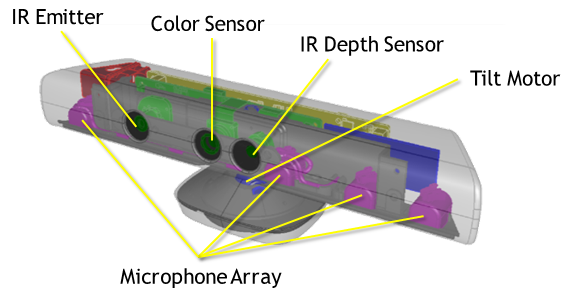
\includegraphics[width=0.8\textwidth]{kinect360_exp}
    \caption{Kinect sensor components. (Image credits: Microsoft\cite{kinect_guide})}
    \label{fig:kinect360_exp}
\end{figure}
%\footnote{\url{https://msdn.microsoft.com/en-us/library/jj131033.aspx}}
Sensor specifications are given in table \ref{tab:kinect}. Note that the range values may differ from what is available in Microsoft's own SDK, as the shortest distance was measured manually in \ac{ROS}. In \cite{kinect_guide}, the depth values for Kinect for Xbox 360 range from $0.8 m$ to $4 m$. Other distances are either unknown, too close or too far away. Kinect for Windows can operate in ''near mode'', i.e. it can measure distances from $0.4 m$ to $3 m$.

\begin{table}
	\centering
	\begin{tabular}{ r | p{6.8cm} }
		\hline
		\multicolumn{2}{c}{Kinect for Xbox 360 Specifications}\\
		\hline
		\textbf{Viewing Angle} & 43° vertical by 57° horizontal field of view. \\
		\hline
		\textbf{Image Resolution} & 640x480 \\
		\hline
		\textbf{FPS} & 30 Hz (given 640x480 depth and color video)\\
		\hline
		\textbf{Minimum Depth} (measured) & $\approx 0.5m$.\\
		\hline
		\textbf{Maximum Depth} & $8 m$.\\
		\hline
		\textbf{Normal (Reliable) Depth Range} & $0.8m < x < 4m$\\
		\hline\hline
	\end{tabular}
	\caption{Kinect for Xbox 360 Specifications.}\label{tab:kinect}
\end{table}


%\begin{figure}[p]
%    \centering
%    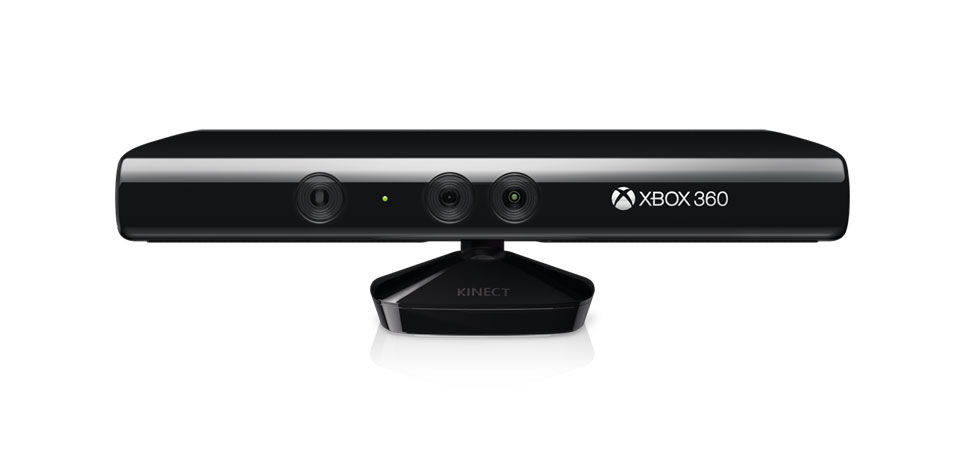
\includegraphics[width=0.8\textwidth]{kinect360}
%    \caption{Awesome Image}
%    \label{fig:kinect360}
%\end{figure}


\subsection{Planar Laser Sensors (LIDAR)}

A planar laser sensor, known as e.g. laser proximity sensors or laser radars, can all be referred to as LIDARs. 

\subsubsection{Scanning Laser Range Finder, URG-04LX-UG01}


\subsection{Odometers}

\subsection{Sensor Fusion}


\section{Simultaneous Localization and Mapping (SLAM)}

\subsection{Introduction to SLAM}

\ac{SLAM}, also known as \ac{CLM}, is a class of solutions to the problem of determining an agents location and pose in an unknown environment, while simultaneously mapping the same environment.

\subsection{Hector SLAM}
\label{sec:hector}
Hector SLAM \cite{KohlbrecherMeyerStrykKlingaufFlexibleSlamSystem2011} is a 2D \ac{SLAM} approach capable of 3D motion estimation. In its original form, the method is suitable for systems with low-end computational power and size, and for mapping of small environments. 2D \ac{SLAM} is based on \ac{LIDAR} scans aligned with the horizontal plane. The full Hector SLAM implementation consist of of a 2D \ac{SLAM} subsystem loosely coupled and synchronized with an \ac{EKF} used as a  6DOF pose estimator. 

The 2D pose of the \ac{LIDAR} is estimated through a scan matcher, i.e. the process of aligning the current \ac{LIDAR} scan with the map generated over the past time steps. The scan matcher was used to provide odometry to \ac{RTAB-Map}, which is the chosen \ac{SLAM} system for this robot. Hector SLAM can be downloaded and used in \ac{ROS} in the form of a prebuild package, \texttt{hector\_slam}.  

\subsection{RTAB-Map}
\label{sec:RTAB-Map}

\ac{RTAB-Map} is developed by IntRoLab at Université de Sherbrooke in Canada. It is a \ac{SLAM} system developed for long term operations in large environments. The system is also intended to handle the ''kidnapped robot-problem'', i.e. multi-session mapping. This is useful whenever the robot is shut down and moved to an unmapped part of the same area, where it will start a new mapping session. \ac{RTAB-Map} is the core feature that has been integrated into the robot described in this thesis. Some factors which motivated the use of \ac{RTAB-Map} are:

\begin{itemize}
	\item It is a \ac{SLAM} method which requires an RGB-D sensor, for example a Kinect. The problem description for this project requires a vision based solution.
	\item \ac{RTAB-Map} has a \ac{ROS} wrapper, \texttt{rtabmap\_ros}, which eases the process of integrating it with the mobile robot.
	\item It includes 3D obstacle detection.
	\item It has a memory management system intended for large scale multi-session mapping.
	\item \ac{RTAB-Map} can be used for object detection. This can be done by linking \ac{RTAB-Map} to OpenCV and the non-free feature detectors \ac{SIFT} and \ac{SURF}.
\end{itemize}

The source code and \ac{ROS} wrapper is currently maintained, and new features and bug-fixes are added regularly. \ac{RTAB-Map} has two distinctive solutions to the \ac{SLAM} problem: Visual loop closure detection and a memory management system for large data sets. The following paragraphs provides an overview of how \ac{RTAB-Map} works. Detailed descriptions of the loop closure detection and memory management approach is provided in  \cite{labbe13appearance}, while the \ac{SLAM} method is presented in \cite{labbe14online}. Further details can be found on the project's Github page\footnote{\url{http://introlab.github.io/rtabmap/}}.

\subsubsection{Graph Based Mapping}

\ac{RTAB-Map} uses a graph structure with nodes and edges to represent the map. New nodes are continuously added to the system's working memory as time passes. In this method, the graph edges are referred to as \textit{links}. There are two types of links: neighbour links and loop closure links. Each node is a location in the map, and the links contain geometrical transformations between the node locations. Figure \ref{fig:rtabmap_graph} illustrated the graph concept.

\begin{figure}[h]
    \centering
    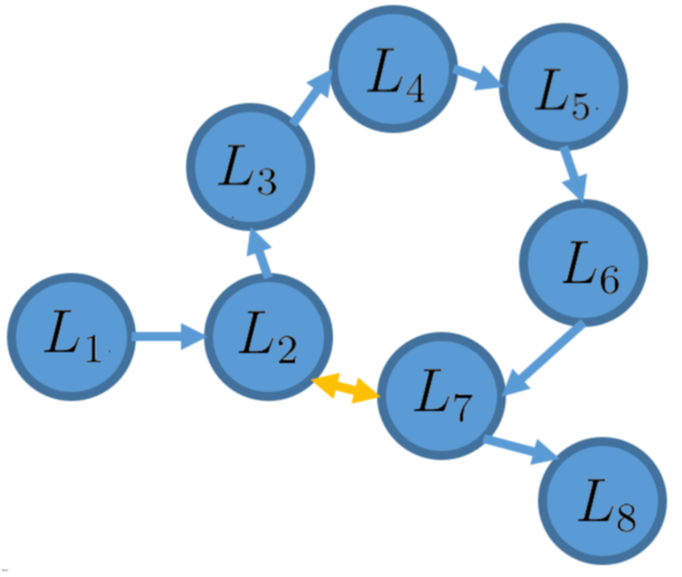
\includegraphics[width=0.5\textwidth]{rtabmap_graph_bl}
    \caption{Conceptual illustration of a graph created by \ac{RTAB-Map} over time $1 \leq t \leq 8 $. A loop closure hypothesis was accepted at $t=7$, as shown by the yellow arrow. Feature descriptors in $L_2$ and $L_7$ are sufficiently similar to accept this as a loop closure.}
    \label{fig:rtabmap_graph}
\end{figure}

\subsubsection{Loop Closure Detection}

\subsubsection{On-line Mapping of Large Environments}



\subsection{RGBD SLAM and Octomap}

Octomap\cite{hornung13auro} is another 3D mapping framework available for \ac{ROS}. Similar to \ac{RTAB-Map}, Octomap can also be used as a standalone version. 

Maps are represented by memory efficient Octrees where each leaf node represents a cube, or voxel, in the volumetric map. The voxel can be either occupied, free or unexplored. The volume of the cube is determined by how deep in the tree the leaf node is located. In a \ac{ROS} graph, the Octomapping is performed by the node \texttt{octomap\_server}. This node  will subscribe to point cloud messages \texttt{sensor\_msgs/PointCloud2}, and return volumetric occupancy maps, i.e. Octomaps.

There are several approaches to \ac{SLAM}  which uses Octomaps. An example that stands out in the context of \ac{ROS} is\cite{endres20143}; a \ac{SLAM} approach which depends on a RGB-D sensor, and relies on Octomap for efficient map storage.

This mapping framework was not used in this project in order to limit the project scope, and because the alternative \ac{RTAB-Map} was associated with less uncertainty.

\section{Autonomous Navigation}

\ac{ROS} provides a pre-built navigation stack for 2D navigation. The navigation stack can plan a path and send velocity commands to the mobile base controller based on sensor input, a goal pose, a map and the frame of the \texttt{base\_link}. Figure \ref{fig:move_base_official} shows how the internal components of the node \texttt{move\_base}, and how it interacts with the rest of the \ac{ROS} system. 

\begin{figure}[h]
    \centering
    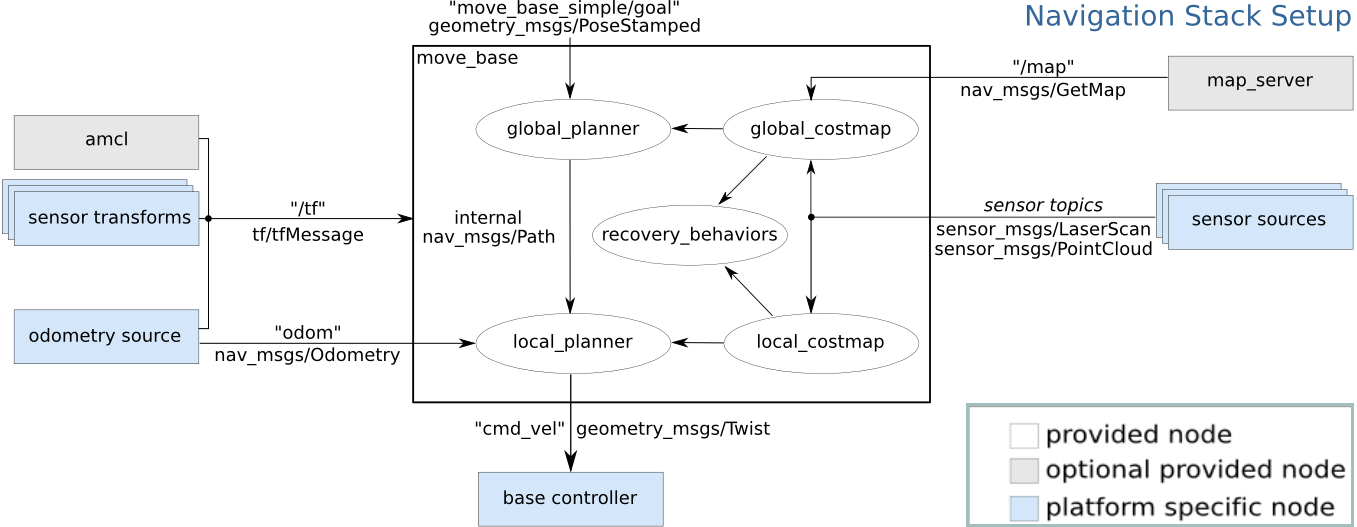
\includegraphics[width=1\textwidth]{move_base_official}
    \caption{\texttt{move\_base} and the navigation stack. (Image credits:  ros.org)}
    \label{fig:move_base_official}
\end{figure}

The navigation stack publishes velocity commands for translation and rotation in the $xy-plane$ in the form of a \texttt{geometry\_msgs/Twist} message with the default topic name ''\texttt{cmd\_vel}''. Mobile bases must constructed as either holonomic or differential drives.

\subsection{Global Planner}

The \ac{ROS} navigation stack is equipped with a basic \textit{global planner}. This global planner is fitted with a set of basic path planning algorithms: e.g. Dijkstra and A*. Global path planning is performed on the global costmap which in turn is based on the 2D grid map published by a map server. A pre-mapped area is not strictly necessary for the global planner to plan a path. Instead it will just plan a naive path which can be corrected by the local planner as the robot moves along the planned trajectory.

\subsection{Local Planner}

Actual velocity commands from \texttt{move\_base} are published by the \textit{local planner}. The local planner will receive the global plan from the global planner, and calculate a new trajectory based on currently observed obstructions as well as the robot footprint and kinematics. Local obstructions are expressed in a dynamic grid map, i.e. the local costmap based, which is based a subset of the global map combined with real time sensor data. The dynamic local cost map enables the robot to avoid temporary and moving obstacles.

The local planner can use either the Trajectory Rollout or \ac{DWA} algorithm for trajectory planning.

\subsection{Recovery Behaviours}

When the robot becomes stuck, it can be configured to perform a set of recovery behaviours. The default recovery behaviours available to \texttt{move\_base} are to clear the costmap, i.e. to remove obstacle information from the costmap, and to rotate in place, in the hope of discovering a new clear path. A typical sequence of behaviours is to clear the costmap, try to locate a path and then attempt an in place rotation before doing a second attempt to plan a path. If the entire series of recovery actions fails to reveal a clear path, the \texttt{move\_base} node will abort and consider the goal state to be infeasible\cite{koubaa2016robot}.